\documentclass{article}
\usepackage{arxiv}

\usepackage[T1]{fontenc}
\usepackage{graphicx}
\usepackage{booktabs}
\usepackage{natbib}
\usepackage{xcolor}
\usepackage[colorlinks=true,linkcolor=teal,citecolor=teal,urlcolor=teal]{hyperref}

% the auto-generated tokens (\TokSpan's en-dash) and refs.bib carry a few Unicode
% typographic glyphs the T1 Times font can't render directly; map them to LaTeX.
\usepackage{newunicodechar}
\newunicodechar{–}{--}
\newunicodechar{—}{---}
\newunicodechar{…}{\ldots}
\newunicodechar{τ}{$\tau$}
\newunicodechar{≤}{$\leq$}
\newunicodechar{≥}{$\geq$}
\newunicodechar{×}{$\times$}

% NOTE on the one warning this build emits and ignores: cairosvg writes the
% chart figures as PDF 1.7, and tectonic's xdvipdfmx defaults its *output* to
% PDF 1.5, so every \includegraphics logs "Trying to include PDF file with
% version (1.7), which is newer than current output PDF setting (1.5)". It is
% cosmetic -- the figures embed and render correctly (they are plain vector
% content, no 1.6/1.7-only features) -- and it is not fixable from here:
% tectonic exposes no output-version flag (`tectonic -Zhelp`), cairosvg exposes
% no target-version argument, `\special{dvipdfmx:config V 7}` is ignored by the
% vendored engine, and no qpdf/gs/mutool is installed to downgrade the figures.
\graphicspath{{figures/}}

% ---------------------------------------------------------------------------
% EVERY corpus statistic in this paper is a \Tok... macro generated by
% scripts/survey_scaffold/tokens_to_tex.py from the exact `tokens` dict that
% builds public/surveys/benchmarks.html — so the PDF and the page cannot state
% different numbers. Never hand-type a corpus number here. The only bare
% numerals in the prose below are (a) values quoted from an individual source
% paper (MT-Bench's 85% judge/human agreement, EvalPlus's 80x test
% densification), which are that paper's numbers and not properties of this
% corpus, (b) schema constants fixed by the taxonomy rather than by the corpus
% (eight facets, six grading families, five horizon rungs, seven kingdoms,
% twenty-five families, nine connections) — written as words — and (c) the
% classification-provenance figures in Section 8, which describe one-time
% historical QA events and are deliberately frozen at the corpus they were run
% against. All three follow the site's own convention, and are stated there
% identically.
% ---------------------------------------------------------------------------
% Auto-generated by scripts/survey_scaffold/tokens_to_tex.py from scripts/benchmarks_survey/build_survey_page.py's computed tokens.
% Do not hand-edit — re-run the script after re-classifying or re-tagging.
\newcommand{\TokN}{369}
\newcommand{\TokSpan}{2000–2026}
\newcommand{\TokSpanYears}{26}
\newcommand{\TokEarliestShort}{TREC-8 QA Track}
\newcommand{\TokEarliestYear}{2000}
\newcommand{\TokLatestShort}{SWE Atlas}
\newcommand{\TokLatestYear}{2026}
\newcommand{\TokNDomains}{16}
\newcommand{\TokNEvalsTag}{86}
\newcommand{\TokNEraLeTwoZeroOneEight}{39}
\newcommand{\TokNEraOneNineTwoZero}{47}
\newcommand{\TokNEraTwoOneTwoTwo}{49}
\newcommand{\TokNTwoZeroTwoThree}{55}
\newcommand{\TokNTwoZeroTwoFour}{85}
\newcommand{\TokNTwoZeroTwoFive}{80}
\newcommand{\TokNTwoZeroTwoSix}{14}
\newcommand{\TokNPreTwoZeroTwoOne}{86}
\newcommand{\TokPctPreTwoZeroTwoOne}{23}
\newcommand{\TokNSat}{69}
\newcommand{\TokNSatPreTwoZeroTwoOne}{47}
\newcommand{\TokPctSatPreTwoZeroTwoOne}{55}
\newcommand{\TokPctSatCorpus}{19}
\newcommand{\TokNPreTwoZeroTwoOneLThreePlus}{2}
\newcommand{\TokPreTwoZeroTwoOneLThreePlusList}{TAPE (2019) and MLPerf Training (2020)}
\newcommand{\TokNKingCap}{202}
\newcommand{\TokPctKingCap}{55}
\newcommand{\TokNKingAudit}{45}
\newcommand{\TokNKingDeploy}{43}
\newcommand{\TokNKingHazard}{26}
\newcommand{\TokNKingWalls}{15}
\newcommand{\TokNKingReward}{8}
\newcommand{\TokNKingMeta}{30}
\newcommand{\TokPctCapPreTwoZeroTwoOne}{74}
\newcommand{\TokPctCapTwoFourTwoFive}{47}
\newcommand{\TokPctCapTwoZeroTwoFive}{41}
\newcommand{\TokNNoncap}{167}
\newcommand{\TokPctNoncap}{45}
\newcommand{\TokFamTop}{A1-perception-parsing}
\newcommand{\TokNFamTop}{57}
\newcommand{\TokNFamAFive}{40}
\newcommand{\TokFamMin}{B1-contamination-twins}
\newcommand{\TokNFamMin}{2}
\newcommand{\TokNFamSmall}{5}
\newcommand{\TokNEmUptoTwoZeroTwoZero}{48}
\newcommand{\TokPctEmLeTwoZeroOneEight}{54}
\newcommand{\TokPctEmTwoZeroTwoFive}{28}
\newcommand{\TokNProgTwoZeroTwoThree}{19}
\newcommand{\TokNProgTwoOneTwoTwo}{19}
\newcommand{\TokPctProgTwoOneTwoTwo}{39}
\newcommand{\TokNProgTwoZeroTwoFive}{29}
\newcommand{\TokPctProgTwoZeroTwoFive}{36}
\newcommand{\TokNLlmjTwoZeroTwoFour}{15}
\newcommand{\TokPctLlmjTwoZeroTwoFour}{18}
\newcommand{\TokEraLlmjPeak}{2024}
\newcommand{\TokGrTopTwoZeroTwoFive}{programmatic}
\newcommand{\TokGrTopTwoZeroTwoFiveN}{29}
\newcommand{\TokGrTopTwoZeroTwoFivePct}{36}
\newcommand{\TokNRubTwoZeroTwoFive}{15}
\newcommand{\TokPctRubTwoZeroTwoFive}{19}
\newcommand{\TokNRubPreTwoZeroTwoFive}{4}
\newcommand{\TokRubPreTwoZeroTwoFiveList}{FActScore (2023), SOTOPIA (2023), TIFA (2023) and Agent-as-a-Judge (2024)}
\newcommand{\TokNRubTwoZeroTwoSix}{3}
\newcommand{\TokRubTwoZeroTwoSixList}{HiL-Bench, MCP-Atlas and SWE Atlas}
\newcommand{\TokRubTwoZeroTwoFiveEx}{HealthBench, MultiChallenge, PaperBench and ToolEyes}
\newcommand{\TokNLOne}{88}
\newcommand{\TokNLThree}{41}
\newcommand{\TokNEmLOne}{54}
\newcommand{\TokNEmLThree}{7}
\newcommand{\TokEmLThreeList}{TAPE, LongICLBench, RULER, AgentDebug, BrowseComp, TRAIL and Who\&When}
\newcommand{\TokNProgLThree}{24}
\newcommand{\TokNProgLFour}{1}
\newcommand{\TokNHumanLFour}{2}
\newcommand{\TokNRubLFour}{1}
\newcommand{\TokPctLThreeTwoZeroTwoThree}{4}
\newcommand{\TokPctLThreeTwoZeroTwoFour}{12}
\newcommand{\TokPctLThreeTwoZeroTwoFive}{28}
\newcommand{\TokPctLThreeTwoZeroTwoSix}{50}
\newcommand{\TokNLThreePlusTwoZeroTwoSix}{7}
\newcommand{\TokNLFour}{4}
\newcommand{\TokLFourList}{BALROG, GDPval, PaperBench and RLI}
\newcommand{\TokLFourYears}{2025}
\newcommand{\TokNLFive}{0}
\newcommand{\TokMeanRungLeTwoZeroOneEight}{1.3}
\newcommand{\TokMeanRungTwoZeroTwoSix}{2.5}
\newcommand{\TokNIe}{96}
\newcommand{\TokFirstIeShort}{ALE}
\newcommand{\TokFirstIeYear}{2013}
\newcommand{\TokNIeOneNineTwoZero}{9}
\newcommand{\TokPctIeLeTwoZeroOneEight}{5}
\newcommand{\TokPctIeOneNineTwoZero}{19}
\newcommand{\TokPctIeTwoOneTwoTwo}{16}
\newcommand{\TokPctIeTwoZeroTwoThree}{16}
\newcommand{\TokPctIeTwoZeroTwoFour}{31}
\newcommand{\TokIeOneNineTwoZeroEx}{Meta-World, Hanabi, RLBench and robosuite}
\newcommand{\TokNIeTwoZeroTwoFive}{33}
\newcommand{\TokPctIeTwoZeroTwoFive}{41}
\newcommand{\TokNIeTwoZeroTwoSix}{9}
\newcommand{\TokPctIeTwoZeroTwoSix}{64}
\newcommand{\TokPctSingleThruTwoZeroTwoZero}{74}
\newcommand{\TokPctSingleTwoZeroTwoSix}{36}
\newcommand{\TokNMultiturn}{35}
\newcommand{\TokPctMultiturnMax}{15}
\newcommand{\TokEraMtPeak}{2018 and earlier}
\newcommand{\TokNMtPreTwoZeroTwoOne}{11}
\newcommand{\TokMtPreTwoZeroTwoOneEx}{DailyDialog, SMN, CMU DoG and PersonaChat}
\newcommand{\TokPctMtTwoZeroTwoFour}{8}
\newcommand{\TokPctMtTwoZeroTwoFive}{8}
\newcommand{\TokNMtTwoZeroTwoSix}{0}
\newcommand{\TokNCrowdexamTwoZeroOneEight}{20}
\newcommand{\TokPctCrowdexamLeTwoZeroOneEight}{51}
\newcommand{\TokPctExpertTwoZeroTwoFive}{48}
\newcommand{\TokPctRwmTwoZeroTwoFive}{10}
\newcommand{\TokPctCrowdTwoZeroTwoFive}{2}
\newcommand{\TokNPrivholdTwoZeroOneEight}{10}
\newcommand{\TokPctPrivholdLeTwoZeroOneEight}{26}
\newcommand{\TokPrivholdLeTwoZeroOneEightEx}{MS COCO, SQuAD, GLUE and HotpotQA}
\newcommand{\TokNNonpubTwoOneTwoTwo}{41}
\newcommand{\TokNonpubTwoOneTwoTwoEx}{Codex, GSM8K, MATH and WebShop}
\newcommand{\TokNPrivholdTwoZeroTwoFive}{22}
\newcommand{\TokPctPrivholdTwoZeroTwoFive}{28}
\newcommand{\TokNDefTwoZeroTwoSix}{6}
\newcommand{\TokPctDefLeTwoZeroOneEight}{28}
\newcommand{\TokPctDefOneNineTwoZero}{19}
\newcommand{\TokPctDefTwoOneTwoTwo}{16}
\newcommand{\TokPctDefTwoZeroTwoThree}{16}
\newcommand{\TokPctDefTwoZeroTwoFour}{25}
\newcommand{\TokPctDefTwoZeroTwoFive}{39}
\newcommand{\TokPctDefTwoZeroTwoSix}{43}
\newcommand{\TokPctDefMax}{43}
\newcommand{\TokNLiverefresh}{12}
\newcommand{\TokNSatLiverefresh}{0}
\newcommand{\TokPctSatPrivhold}{23}
\newcommand{\TokPctSatLOne}{44}
\newcommand{\TokPctSatLTwo}{12}
\newcommand{\TokPctSatLThreePlus}{2}
\newcommand{\TokNSatLThreePlus}{1}
\newcommand{\TokSatLThreePlusList}{TAPE (2019)}
\newcommand{\TokNLTwo}{236}
\newcommand{\TokPctClosingLTwo}{17}
\newcommand{\TokPctOpenLThreePlus}{73}
\newcommand{\TokNEdges}{2013}
\newcommand{\TokGravHumaneval}{66}
\newcommand{\TokGravApps}{20}
\newcommand{\TokNIeCross}{31}
\newcommand{\TokGravTop}{Codex}
\newcommand{\TokGravTopN}{66}
\newcommand{\TokGravRunnerup}{MMLU}
\newcommand{\TokGravRunnerupN}{63}
\newcommand{\TokNLineage}{682}
\newcommand{\TokNCorrections}{48}
\newcommand{\TokLagMedLeTwoZeroOneEight}{3}
\newcommand{\TokLagMaxLeTwoZeroOneEight}{10}
\newcommand{\TokLagMedOneNineTwoZero}{4}
\newcommand{\TokLagMaxOneNineTwoZero}{5}
\newcommand{\TokLagMedTwoOneTwoTwo}{2.5}
\newcommand{\TokLagMaxTwoOneTwoTwo}{3}
\newcommand{\TokLagMedTwoThreeTwoFour}{1}
\newcommand{\TokLagMaxTwoThreeTwoFour}{2}
\newcommand{\TokNAudited}{32}
\newcommand{\TokLagMax}{10}
\newcommand{\TokLagMaxPair}{ImageNet $\rightarrow$ ImageNet-C/P}
\newcommand{\TokNTopTwoZeroAudited}{12}
\newcommand{\TokTopTwoZeroUnauditedEx}{SuperGLUE, WebShop, AgentBench and Gorilla}
\newcommand{\TokSwelDescList}{GDPval, RLI and UpBench}
\newcommand{\TokNSwelDescCoding}{0}
\newcommand{\TokNConfMed}{151}
\newcommand{\TokNDomVocab}{17}


\title{The Anatomy of a Benchmark: A Role Taxonomy of \TokN{} AI Evaluation
Benchmarks and the Grading Economics That Bounds Them}

\author{Darvin Yi\thanks{Companion to the live, interactive survey at
\url{https://research.darvinyi.com/surveys/benchmarks.html}, from which the corpus,
every figure, and every statistic in this paper are generated. This preprint is a
condensation of that page; where a number appears here it is the same value the page
computes from the classified corpus.} \\
\texttt{research.darvinyi.com}}

\date{August 2026}

\begin{document}
\maketitle

\begin{abstract}
We survey \TokN{} artificial-intelligence evaluation benchmarks spanning \TokSpan{} ---
from \TokEarliestShort{} (\TokEarliestYear{}) to \TokLatestShort{} (\TokLatestYear{}) ---
each read individually and then classified along eight facets: domain, task shape, grading
family, task horizon, tool access, provenance, contamination defense, and saturation. It is
not an LLM-era corpus: \TokNPreTwoZeroTwoOne{} of the \TokN{} papers
(\TokPctPreTwoZeroTwoOne\%) were published before 2021, which lets era-level trends be read
over a quarter-century of measurement practice rather than over three years of it. Instead of
sorting benchmarks by \emph{what} they measure, we place each at a single address in a
taxonomy of seven \emph{kingdoms} defined by the question a benchmark was built to answer at
its birth. Capability probes --- the thing ``benchmark'' is usually taken to mean --- are a
bare majority of the whole corpus (\TokNKingCap{} of \TokN{}, \TokPctKingCap\%) but a clear
minority of its present (\TokPctCapTwoZeroTwoFive\% of 2025 entries), as the field turns to
auditing its own measurements, rehearsing deployments, probing hazards, and manufacturing
training signal. Our organizing thesis is a grading-economics constraint: \emph{a benchmark
can only pose tasks as long as it can afford to grade them}. Cheap, mechanical grading thins
out as task horizons lengthen, so the reach of evaluation is bounded by the cost of its
grader, and a benchmark's expected lifespan is bought in human-minutes per item. We support
this with seven findings read off cross-tabulations by publication era --- among them that
the interactive turn is a \emph{return} rather than an arrival (the corpus's first
interactive environment is \TokFirstIeShort{}, \TokFirstIeYear{}), that rubric grading is
2025's fastest-growing but not its largest grading family, and that no era in
\TokSpanYears{} years has shipped a contamination defense on as much as half of its new
benchmarks --- and close with three cross-paper connections visible only across papers.
\end{abstract}

\keywords{benchmarks \and evaluation \and large language models \and agents \and taxonomy \and contamination \and reward hacking}

\section{Introduction}

Read one benchmark paper and you learn a benchmark: its task, its metric, its headline
score. Read all of them at once and a different object comes into view --- an ecosystem of
instruments that measure each other, feed each other's training, and decay on a schedule.
This survey takes \TokN{} AI evaluation benchmarks, each already read and summarized as an
individual explainer, and asks what the collection shows that no single paper can.

We include a paper when a named benchmark, evaluation dataset, or evaluation environment
is its \textbf{headline contribution} --- the thing a survey would cite it for. Models,
training methods, and agent frameworks that merely \emph{report} benchmark numbers are
excluded. That rubric yields \TokN{} papers spanning \TokSpan{}.
\TokNEvalsTag{} of them additionally shipped a new \emph{way} to evaluate alongside their
data --- an Elo protocol, a scenario grid, an atomic-fact decomposition --- and so also
carry an \texttt{evaluations} tag in the underlying atlas.

The corpus is curated rather than exhaustive, but it is not confined to the language-model
era: \TokNPreTwoZeroTwoOne{} of the \TokN{} papers (\TokPctPreTwoZeroTwoOne\%) predate 2021,
and they are present as a subject, not as ancestry. They include the question-answering and
dialogue generations that precede the LLM era (\TokEarliestShort{} in \TokEarliestYear{},
PASCAL RTE~\citep{dagan-2005-rte}, DailyDialog~\citep{li-2017-dailydialog},
PersonaChat~\citep{zhang-2018-personachat}), the vision canon
(ImageNet~\citep{deng-2009-imagenet}, CIFAR-10/100~\citep{krizhevsky-2009-cifar},
MS COCO~\citep{lin-2014-coco}, VQA~\citep{antol-2015-vqa}), a deep-reinforcement-learning
and robotics block (\TokFirstIeShort{} in \TokFirstIeYear{},
OpenAI Gym~\citep{brockman-2016-openai-gym}, \TokIeOneNineTwoZeroEx{}), multi-agent game
environments, speech, and a text-to-image and text-to-video evaluation cluster. That older
block prefigures the shape of today's agent benchmarks largely \emph{without} a citation
path to them (Section~\ref{sec:shape}), which is a finding the LLM-only view of this
literature cannot produce.

Existing surveys of AI evaluation sit on two shelves that barely touch. One taxonomizes
\emph{what benchmarks measure} --- organizing the field by task type, by evaluated property,
or, most rigorously, by a scenario-by-metric grid the survey then deliberately fills, as in
HELM~\citep{liang-2022-helm}. The other grades \emph{how well benchmarks are built}:
lifecycle scorecards, integrity reviews, construct-validity audits across hundreds of
benchmarks, and the agentic-benchmark checklist that found unsound graders in 7 of 10 suites
it audited. The agent-evaluation surveys of 2025 added structural vocabulary --- dataset
versus environment, offline versus online, tool access --- but each coins its own terms and
none quantifies the axes it names. What no prior survey does is \textbf{cross the shelves at
the level of the individual paper}: place every benchmark in a capability map \emph{and}
record its grading machinery, task horizon, tool surface, provenance, and contamination
posture, then read the joint distribution over time. That cross is this survey's
contribution, on a corpus that is densely annotated rather than merely enumerated --- every
paper here has been read, summarized, and critiqued individually, and the underlying
citation graph is browsable as a timeline.

The dimension that turns out to organize the most --- \emph{how long the task is} --- was
made measurable only recently, by time-horizon work reporting a roughly seven-month doubling
of frontier models' 50\%-success horizon, and has never before been applied to a benchmark
corpus. It also reconciles this corpus with the recent finding that roughly half of all
benchmarks are saturated. Here the pre-2021 cohort is saturated at \TokPctSatPreTwoZeroTwoOne\%
(\TokNSatPreTwoZeroTwoOne{} of \TokNPreTwoZeroTwoOne{}) against \TokPctSatCorpus\%
corpus-wide, and the reason is horizon rather than age: all but
\TokNPreTwoZeroTwoOneLThreePlus{} of those \TokNPreTwoZeroTwoOne{} early papers pose a task
a human expert finishes inside half an hour, the exceptions being
\TokPreTwoZeroTwoOneLThreePlusList{}.

\section{The corpus and its facets}
\label{sec:facets}

Each of the \TokN{} papers was classified along eight facets, each a question with a closed
answer set. Six are descriptive and we treat them briefly: \emph{domain} (what capability is
chiefly measured); \emph{task shape} (single-turn, multi-turn dialogue, or interactive
environment); \emph{tool access} (what the evaluated model may touch --- nothing, a code
interpreter, a browser, a whole operating system); \emph{provenance} (where the task items
came from); \emph{contamination defense} (the strongest mechanism keeping items out of
training sets); and \emph{saturation} (whether headroom remains, judged from the frontier
scores each explainer quotes). Two facets do enough analytical work to deserve their own
definitions, and together they carry the paper's thesis.

One limit of the domain facet should be stated before any domain-conditioned claim is read.
Its vocabulary was designed for a corpus of language-model and agent evaluation, and the
corpus outgrew it: robotics and manipulation are recorded as \texttt{multimodal}, multi-agent
reinforcement learning and games as \texttt{reasoning}, theory of mind as
\texttt{social-moral}. \TokNDomains{} of the vocabulary's \TokNDomVocab{} values are actually
used, and the affected papers are real members of the corpus rather than strays --- the
embodied-operation family alone holds \TokNFamAFive{} of them. Every affected record says so
in its notes; read the domain values as ``nearest available label.''

\paragraph{Task horizon.} ``Complexity'' is the word everyone reaches for and nobody
defines; the literature operationalizes it at least five incommensurable ways --- reasoning
steps, compositional depth, context length, search-space size, item-response difficulty ---
none of which lets you compare a multiple-choice exam to a week of freelance software work.
We use the one currency that spans the whole corpus: the \textbf{wall-clock time a competent
human domain-expert would need to complete one \emph{typical} task instance}, reading and
artifact production included. This is the axis along which frontier ability was shown to
climb at a measurable rate, and it sorts the corpus into five rungs
(Figure~\ref{fig:ladder}): \textbf{L1} under one minute, \textbf{L2} one to thirty minutes,
\textbf{L3} thirty minutes to a day, \textbf{L4} a day to two weeks, and \textbf{L5} beyond
two weeks. Only a handful of papers (GDPval~\citep{patwardhan-2025-gdpval}, the METR suites)
actually \emph{measure} human time; elsewhere the rung is estimated from the paper's own task
descriptions.

\begin{figure}[t]
  \centering
  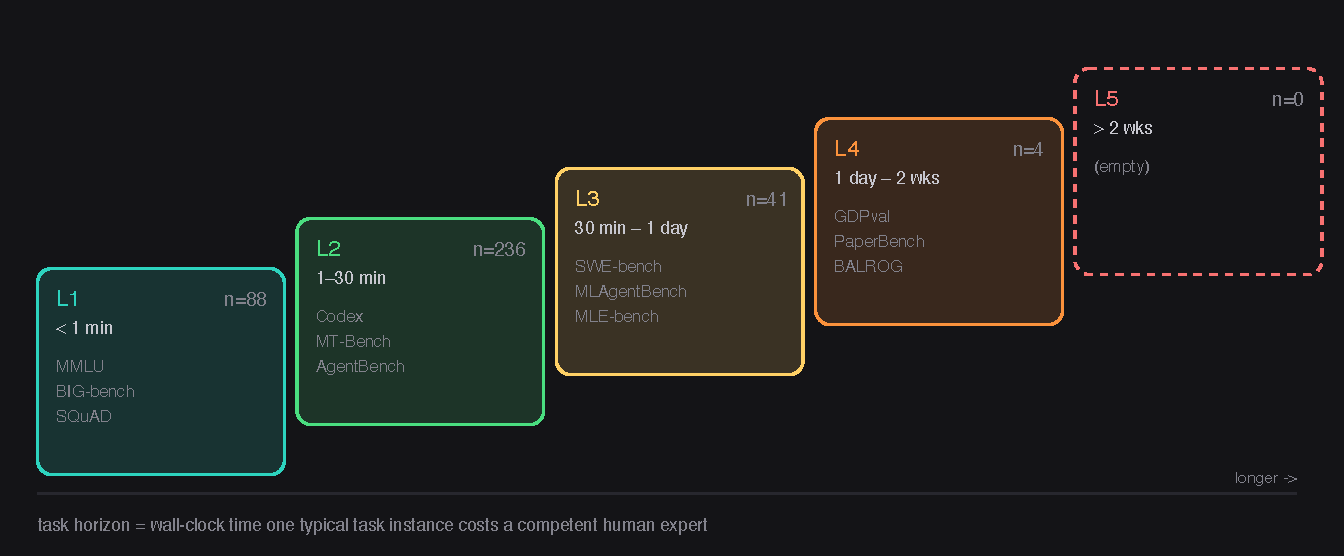
\includegraphics[width=\textwidth]{ladder.pdf}
  \caption{The horizon ladder: count and canonical examples per rung across all \TokN{}
  papers. The examples are each rung's three most-cited members, read off the corpus rather
  than chosen by hand. \TokNLTwo{} of the \TokN{} papers sit at L2, and the top rung holds
  \TokNLFive{}.}
  \label{fig:ladder}
\end{figure}

\paragraph{Grading family.} Every benchmark answers ``who says the output is right?'' with
one of six mechanisms, and the choice is less methodological free will than economics
(Figure~\ref{fig:grladder}). Ordered by the cost to grade a single item, they run:
\emph{proxy metric} (BLEU/ROUGE-style scores, now largely distrusted and sitting outside the
ladder), \emph{exact match} (the answer key is the grader, effectively free),
\emph{programmatic} (unit tests, checkers, environment end-states --- build a harness once),
\emph{LLM judge} (one holistic model call), \emph{rubric + judge} (experts author per-item
criteria a model then applies), and \emph{human} (expert or preference grading, at
expert-hours per item). Each step up the ladder buys generality --- the ability to grade more
open-ended work --- and pays for it in cost per item and in grader error that must itself be
audited.

\begin{figure}[t]
  \centering
  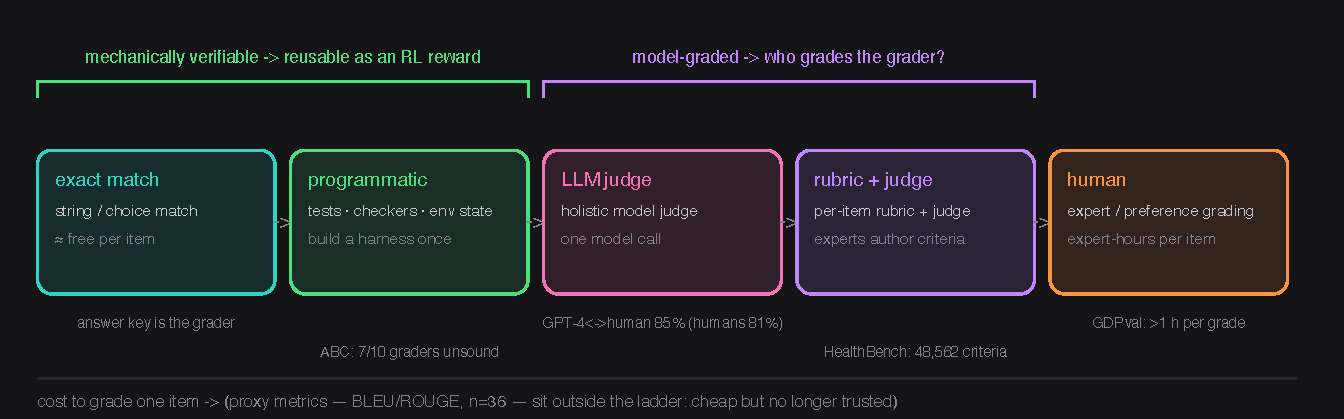
\includegraphics[width=\textwidth]{grladder.pdf}
  \caption{The grading-cost ladder, ordered by what it costs to grade one item. The
  reliability annotations are the source papers' own: MT-Bench measured GPT-4-judge/human
  agreement at 85\% (humans agree with each other 81\%); the agentic-benchmark checklist
  found unsound graders in 7 of 10 suites. The two brackets mark the mechanically verifiable
  families (reusable as RL rewards) and the model-graded families (which raise the question
  of who grades the grader).}
  \label{fig:grladder}
\end{figure}

Two structural notes follow from this ladder. First, its cheap end is exactly what the era
of reinforcement learning with verifiable rewards trains on: a benchmark whose grader is
mechanical is also a reward function, so the most verifiable benchmarks are precisely the
ones models are optimized against. Goodhart exposure is a property of the grading family,
not of the dataset. Second, the model-graded middle opened a regress the field is still
funding --- judges are now themselves benchmarked by meta-benchmarks such as
RewardBench~\citep{lambert-2024-rewardbench} and JudgeBench~\citep{tan-2024-judgebench}, and
rubric grading is the current attempt to make judge error inspectable by decomposing it into
checkable criteria.

\paragraph{The corpus has edges.} Four papers in it are, on inspection, not benchmark papers
by the rubric of Section~\ref{sec:intro-rubric}, and saying so is more useful than quietly
dropping them. MLPerf Training~\citep{mattson-2020-mlperf-training} measures hardware and
software throughput to a fixed accuracy gate; LCCC~\citep{wang-2020-lccc} and
MedDialog~\citep{chen-2020-meddialog} are pretraining corpora whose only evaluation runs on
someone else's benchmark; AgentSkillOS~\citep{li-2026-agentskillos} grades an unnamed
thirty-task benchmark with models from the same family that produced the answers. The tell
was mechanical and it generalizes: for MLPerf the classifier reported that \emph{every}
facet was a forced choice. \textbf{When every facet of a record is a forced choice, the
schema is telling you the paper is not the kind of object the schema describes.} They remain
in every count below; where one of them is the reason a cell is non-empty, we say so.

\section{A taxonomy by evolutionary role}
\label{sec:tree}

Sorting benchmarks by what they test merely reproduces the domain facet. Sorting them by
\emph{why they exist} produces a different --- and, we argue, more honest --- structure. The
placement question is: \textbf{what question was this benchmark built to answer, in the
ecosystem of models and benchmarks that existed at its birth?} Judged from each paper's own
problem statement, that question has seven answers --- seven \emph{kingdoms} --- and every
one of the \TokN{} papers sits at exactly one address. The kingdoms subdivide into
twenty-five families; Figure~\ref{fig:tree} shows the whole tree and Table~\ref{tab:kingdoms}
its top level.

\begin{figure}[t]
  \centering
  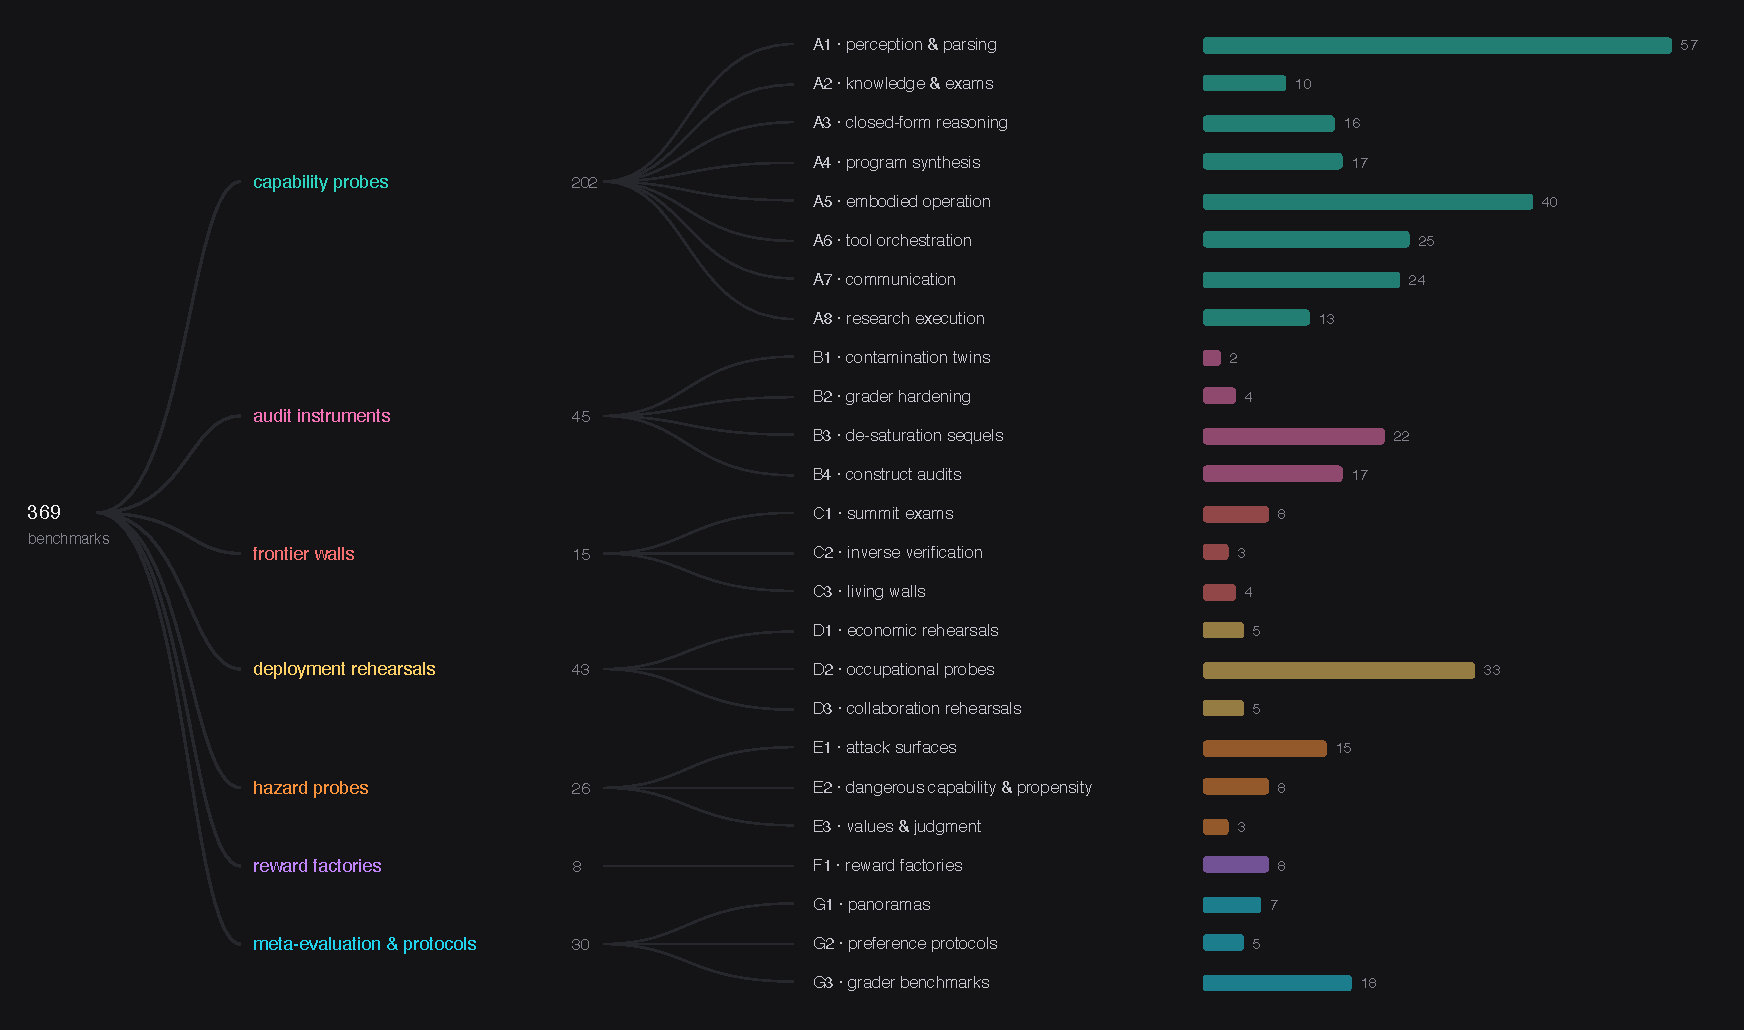
\includegraphics[width=\textwidth]{tree.pdf}
  \caption{The role taxonomy: seven kingdoms, twenty-five families, \TokN{} leaves. Bars are
  family sizes. Placement is by role at birth, not later use, so HellaSwag sits under
  de-saturation sequels (kingdom B) rather than commonsense reasoning, and SWE-bench sits
  under program synthesis (kingdom A) rather than agents.}
  \label{fig:tree}
\end{figure}

\begin{table}[t]
  \centering
  \small
  \begin{tabular}{clcl}
    \toprule
    & \textbf{Kingdom} & \textbf{\#} & \textbf{The question it was built to answer} \\
    \midrule
    A & capability probes           & \TokNKingCap{}    & Can models do X yet? \\
    B & audit instruments           & \TokNKingAudit{}  & Is our measurement lying? \\
    C & frontier walls              & \TokNKingWalls{}  & Can we build something that stays unsolved? \\
    D & deployment rehearsals       & \TokNKingDeploy{} & What happens when we ship it into this job? \\
    E & hazard probes               & \TokNKingHazard{} & What could go wrong? \\
    F & reward factories            & \TokNKingReward{} & Can the benchmark generate its own training signal? \\
    G & meta-evaluation \& protocols & \TokNKingMeta{}   & How should we evaluate at all? \\
    \bottomrule
  \end{tabular}
  \caption{The seven kingdoms, their sizes, and the one-line question each answers.}
  \label{tab:kingdoms}
\end{table}

The tree's shape is a finding in its own right, and the shape is lopsided and tilting.
\TokNKingCap{} of the \TokN{} papers (\TokPctKingCap\%) are capability probes --- benchmarks
that ask ``can the model do X?'' --- but that bare majority is an artifact of the corpus's
history rather than of its present. Capability probes are \TokPctCapPreTwoZeroTwoOne\% of
pre-2021 entries, \TokPctCapTwoFourTwoFive\% of 2024--25 entries, and
\TokPctCapTwoZeroTwoFive\% of 2025 alone, where they are a clear minority. The other
\TokNNoncap{} papers (\TokPctNoncap\%) do something more reflexive: audit other measurements
(\TokNKingAudit{}), rehearse deployments (\TokNKingDeploy{}), probe hazards
(\TokNKingHazard{}), build walls designed not to fall (\TokNKingWalls{}), manufacture
training signal (\TokNKingReward{}), or work out how to evaluate at all (\TokNKingMeta{}).
Benchmarking has become an ecosystem with predators, parasites, and decomposers --- not a
row of thermometers.

The families are lopsided too, and in a way that dates the corpus. The largest is
\texttt{\TokFamTop{}} at \TokNFamTop{} papers --- recognize, parse, entail, retrieve --- the
pre-LLM vision-and-language-understanding stratum sitting under everything else. The second
largest, \texttt{A5-embodied-operation} at \TokNFamAFive{}, spans two generations that share
a form more than a bibliography: deep-RL and robotics environments from \TokFirstIeYear{}
onward, then LLM agent environments from 2022 (Section~\ref{sec:shape}). At the other end,
\TokNFamSmall{} families hold fewer than five papers each, the smallest being
\texttt{\TokFamMin{}} at \TokNFamMin{}. Small families are not noise: rebuilding a
benchmark's test set from scratch to measure overfitting is expensive work few teams do, so
the size of the contamination-twin family is a fact about cost, not about whether the
question is settled.

Placement is by role at birth, not later use, which is what makes the taxonomy informative
rather than a restatement of topic. HellaSwag~\citep{zellers-2019-hellaswag} sits among the
de-saturation sequels because it was built to resurrect a solved benchmark, and its
adversarial-filtering construction matters more than its commonsense content.
SWE-bench~\citep{jimenez-2023-swe-bench} sits under program synthesis because the agents came
later. GSM8K~\citep{cobbe-2021-gsm8k} sits under closed-form reasoning even though its
deepest legacy is the verifier paradigm (Section~\ref{sec:reward}). The tree records what
each benchmark was \emph{for}, and it is the reflexive kingdoms --- B, C, F, G --- that a
topic-based taxonomy renders invisible.

\section{Findings}
\label{sec:findings}

Seven findings, each read off a cross-tabulation of the corpus by publication era. Per-era
counts are small enough that these should be read as slopes, not decimals; the eras pool
sparse early years (\TokNEraLeTwoZeroOneEight{} papers through 2018,
\TokNEraOneNineTwoZero{} in 2019--20, \TokNEraTwoOneTwoTwo{} in 2021--22) and break out
single years thereafter (\TokNTwoZeroTwoThree{}, \TokNTwoZeroTwoFour{},
\TokNTwoZeroTwoFive{}, and \TokNTwoZeroTwoSix{} papers for 2023 through 2026).

\subsection{The grading waves, and the 2025 rubric turn}
\label{sec:waves}

\begin{figure}[t]
  \centering
  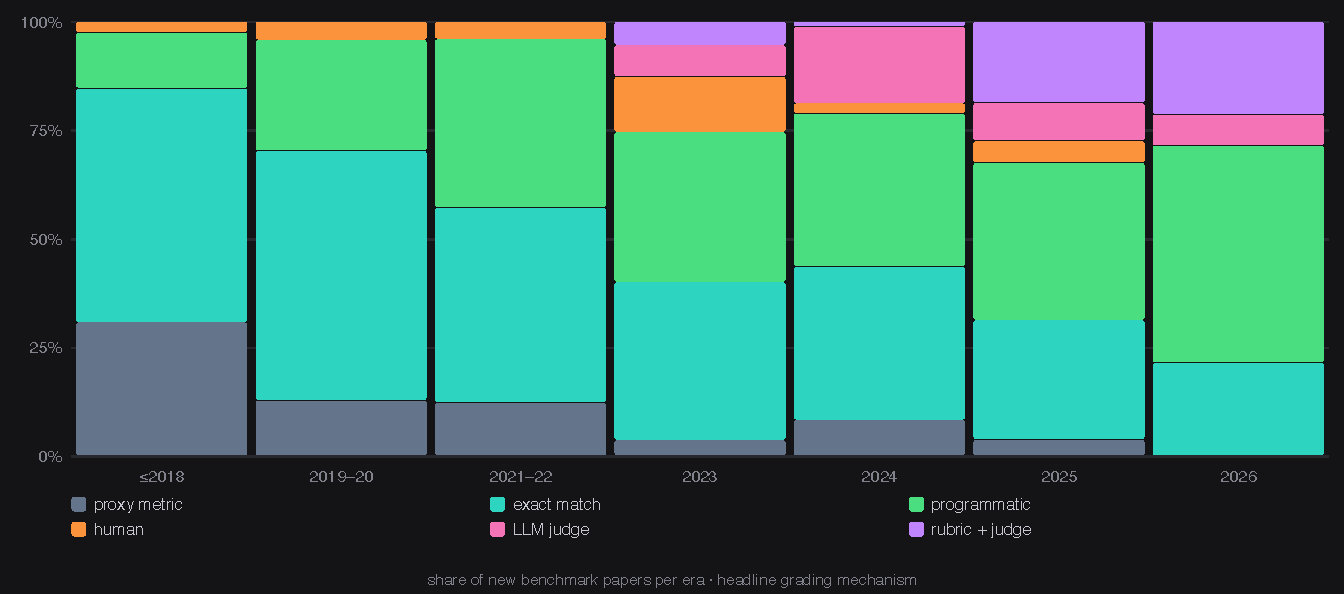
\includegraphics[width=\textwidth]{waves.pdf}
  \caption{Headline grading mechanism by era, as a share of each era's new benchmark papers.}
  \label{fig:waves}
\end{figure}

Grading moves in waves, and each wave displaces the one before it rather than replacing it
outright (Figure~\ref{fig:waves}). Proxy metrics gave way to exact match, which owned the
early corpus --- \TokPctEmLeTwoZeroOneEight\% of papers through 2018,
\TokNEmUptoTwoZeroTwoZero{} of \TokNPreTwoZeroTwoOne{} up to 2020 --- and has fallen every
era since, to \TokPctEmTwoZeroTwoFive\% in 2025. Execution-based programmatic grading arrived
with the code and environment benchmarks (\TokNProgTwoOneTwoTwo{} of \TokNEraTwoOneTwoTwo{}
in 2021--22, \TokPctProgTwoOneTwoTwo\%) and has held about a third of every cohort since:
\textbf{the largest grading family for new benchmarks in 2025 is \TokGrTopTwoZeroTwoFive{}},
at \TokGrTopTwoZeroTwoFiveN{} of \TokNTwoZeroTwoFive{} (\TokGrTopTwoZeroTwoFivePct\%).
Holistic LLM-judging peaked in \TokEraLlmjPeak{} (\TokNLlmjTwoZeroTwoFour{} papers,
\TokPctLlmjTwoZeroTwoFour\%) and has receded since.

The genuinely new wave is rubric-scored judging, and \textbf{its slope is the story rather
than its size}: \TokNRubPreTwoZeroTwoFive{} papers \emph{total} before 2025
(\TokRubPreTwoZeroTwoFiveList{}), then \TokNRubTwoZeroTwoFive{} of \TokNTwoZeroTwoFive{}
(\TokPctRubTwoZeroTwoFive\%) in a single year --- \TokRubTwoZeroTwoFiveEx{} among them ---
and \TokNRubTwoZeroTwoSix{} of \TokNTwoZeroTwoSix{} in 2026 (\TokRubTwoZeroTwoSixList{}). Set
against \TokGrTopTwoZeroTwoFiveN{} new \TokGrTopTwoZeroTwoFive{} benchmarks in the same year,
that is a turn, not a takeover. We flag this explicitly because it is where a smaller corpus
misleads: read on 139 papers, rubric judging looked like 2025's largest grading family, and
the fuller corpus falsifies that.

The wave structure has a single driver: each new capability regime produced outputs the
previous grader could not score. Exact match broke on free-form generation; unit tests broke
on anything that is not code; holistic judges broke on expert domains where ``sounds good''
diverges from ``is correct.'' The rubric turn is the field's current answer --- decompose
expert judgment into criteria a model \emph{can} check --- and it is also a quiet confession
that the thing we now want to measure no longer has an answer key. That the mechanical
families still grade most new benchmarks says the field has not abandoned verifiability; it
has partitioned, sending checkable work to harnesses and open-ended work to rubrics.

\subsection{The verifiability frontier}
\label{sec:frontier}

\begin{figure}[t]
  \centering
  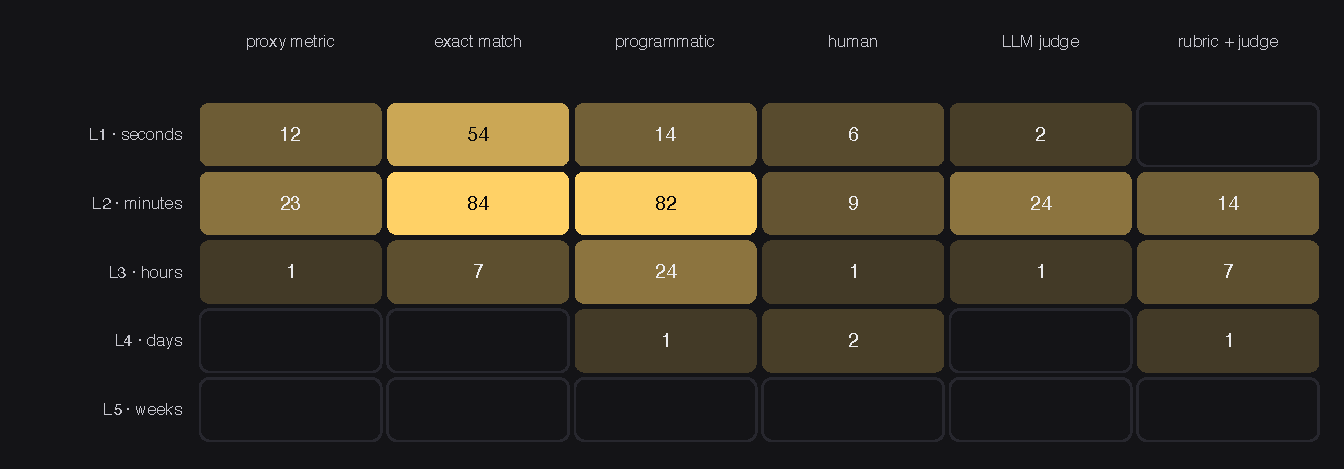
\includegraphics[width=\textwidth]{frontier.pdf}
  \caption{Task horizon $\times$ grading family, all \TokN{} papers; hollow cells are empty.
  The mechanical families thin out with horizon but do not die: \TokNEmLThree{} exact-match
  and \TokNProgLThree{} programmatic papers survive at L3, and L4 is split
  \TokNHumanLFour{} human, \TokNRubLFour{} rubric, \TokNProgLFour{} programmatic.}
  \label{fig:frontier}
\end{figure}

Read Figure~\ref{fig:frontier} diagonally and a boundary appears: \textbf{cheap grading gets
rarer as horizons lengthen, and it survives only where the answer stays short}. Exact match
owns L1 (\TokNEmLOne{} of the \TokNLOne{} L1 papers) and thins to \TokNEmLThree{} of
\TokNLThree{} at L3 --- \TokEmLThreeList{} --- none of which is a general-purpose answer key.
They are short keys bolted onto long work: needle retrieval inside a very long context,
search questions inverted until the answer is a verifiable string, and error localization in
a recorded agent trace against a fixed label set. Programmatic grading peaks at L2--L3
(\TokNProgLThree{} papers: unit tests, environment end-states) and nearly disappears at L4,
where it survives in \TokNProgLFour{} paper --- a game environment whose end state is still
machine-readable. Nobody has built a test harness for ``produce a competitive research
paper.''

This is the survey's central claim: \textbf{a benchmark can only pose tasks as long as it
can afford to grade them.} Verification asymmetry --- tasks that are hard to do but cheap to
check --- is the scarce resource of benchmark design, and the L4 row shows what happens when
it runs out. GDPval pays experts for more than an hour of pairwise grading per item;
PaperBench~\citep{starace-2025-paperbench} amortizes thirty-three person-weeks of rubric
authoring. The grading-cost ladder of Section~\ref{sec:facets} is not a menu of equally
available options; at high horizons it is a budget constraint.

\subsection{The horizon climb, and the empty top rung}

\begin{figure}[t]
  \centering
  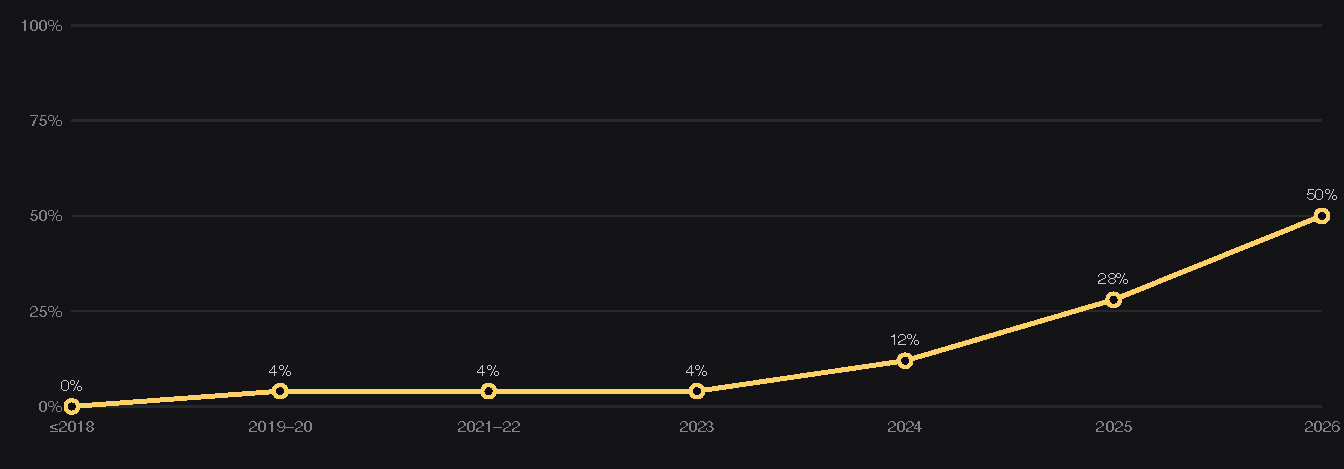
\includegraphics[width=\textwidth]{climb.pdf}
  \caption{Share of each era's new benchmark papers posing L3+ tasks ($\geq$30 expert-minutes
  per instance).}
  \label{fig:climb}
\end{figure}

Benchmarks are climbing the same ladder their subjects climb (Figure~\ref{fig:climb}). In
the corpus's first two decades only \TokNPreTwoZeroTwoOneLThreePlus{} papers posed a task
above L2 --- \TokPreTwoZeroTwoOneLThreePlusList{}, and one of those, MLPerf, is a throughput
harness rather than a capability eval. The L3+ share was
\TokPctLThreeTwoZeroTwoThree--\TokPctLThreeTwoZeroTwoFour\% through 2023--24, then jumped to
\TokPctLThreeTwoZeroTwoFive\% in 2025 and reached \TokNLThreePlusTwoZeroTwoSix{} of
\TokNTwoZeroTwoSix{} papers in 2026 (\TokPctLThreeTwoZeroTwoSix\%); the mean rung moved from
\TokMeanRungLeTwoZeroOneEight{} ($\leq$2018) to \TokMeanRungTwoZeroTwoSix{} (2026). That
tracks the measured capability curve: as a model's 50\%-success horizon doubles roughly every
seven months, benchmarks below the frontier stop discriminating and the field rebuilds one
rung up.

But the climb is running out of ladder. L4 --- day-to-week projects --- contains
\TokNLFour{} papers (\TokLFourList{}), all from \TokLFourYears{}, and \textbf{L5 holds
\TokNLFive{}}: no benchmark in this corpus poses work beyond two expert-weeks. The binding
constraints are the two graders left at that altitude (Section~\ref{sec:frontier}) and item
economics --- a thousand-item benchmark of week-long tasks is a thousand expert-weeks of
ground truth. Whoever solves cheap verification of long-horizon work gets to write the first
L5 benchmark, and probably the reward signal for the next training era with it.

\subsection{The interactive turn is a return, and multi-turn dialogue is what got dropped}
\label{sec:shape}

\begin{figure}[t]
  \centering
  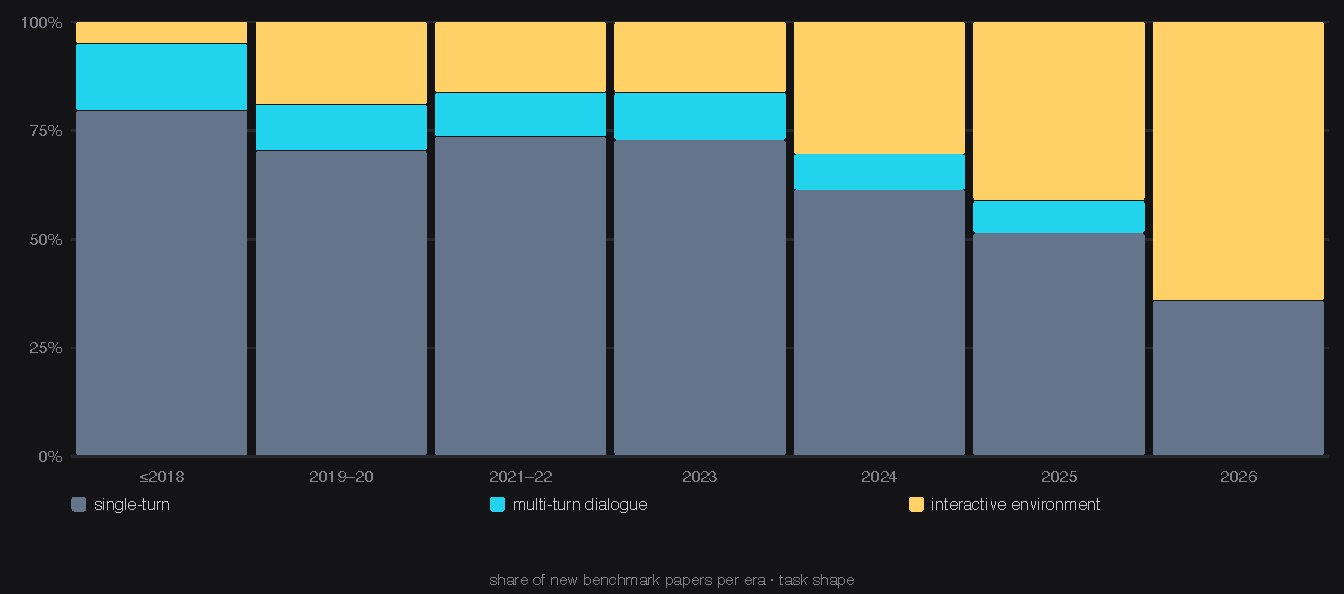
\includegraphics[width=\textwidth]{shape.pdf}
  \caption{Task shape by era. Interactive environments: the model acts, the environment
  responds, repeat. Multi-turn: dialogue without an environment.}
  \label{fig:shape}
\end{figure}

Interactive environments are not new here, and reading the recent climb as an invention is
the mistake a smaller corpus invites. The first one is \TokFirstIeShort{}
(\TokFirstIeYear{})~\citep{bellemare-2013-ale}, and the 2019--20 cohort is already
\TokPctIeOneNineTwoZero\% interactive (\TokNIeOneNineTwoZero{} papers,
\TokIeOneNineTwoZeroEx{} among them) --- but that block evaluates \emph{policies}, in
robotics simulators and multi-agent games. The two generations do touch: \TokNIeCross{}
in-corpus citations run between them. They run through robotics and games, though ---
LIBERO~\citep{liu-2023-libero} and ManiSkill2~\citep{gu-2023-maniskill2} citing
RLBench~\citep{james-2020-rlbench} and Meta-World~\citep{yu-2019-meta-world},
BALROG~\citep{paglieri-2024-balrog} citing \TokFirstIeShort{} --- and not through the
web-and-tool environments that drive the recent climb, which descend from
WebShop~\citep{yao-2022-webshop} rather than from Gym.

The language-model era, in other words, did not inherit the form: the interactive share sits
at \TokPctIeTwoOneTwoTwo\% in 2021--22 and \TokPctIeTwoZeroTwoThree\% in 2023, still mostly
simulators and games, with WebShop the language-agent beachhead in 2022. Only then does it
climb, on a different lineage: \TokPctIeTwoZeroTwoFour\% in 2024,
\TokPctIeTwoZeroTwoFive\% in 2025 (\TokNIeTwoZeroTwoFive{} of \TokNTwoZeroTwoFive{}),
\TokPctIeTwoZeroTwoSix\% in 2026 (\TokNIeTwoZeroTwoSix{} of \TokNTwoZeroTwoSix{}). The static
single-turn dataset was \TokPctSingleThruTwoZeroTwoZero\% of the corpus through 2020 and is
\TokPctSingleTwoZeroTwoSix\% of 2026, already the minority format. The migration the agent
surveys narrate is real; what the full timeline adds is that the field \emph{re-derived} a
form it had abandoned, from different ancestors.

The anomaly is what got dropped. \textbf{Multi-turn dialogue is \TokNMultiturn{} papers out
of \TokN{}}, and its high-water mark is the \emph{oldest} era in the corpus
(\TokEraMtPeak{}, \TokPctMultiturnMax\%), when dialogue systems were the product and
\TokNMtPreTwoZeroTwoOne{} pre-2021 papers evaluated conversation directly
(\TokMtPreTwoZeroTwoOneEx{}). No era since has matched that share:
\TokPctMtTwoZeroTwoFour\% in 2024, \TokPctMtTwoZeroTwoFive\% in 2025,
\TokNMtTwoZeroTwoSix{} papers in 2026. The field did not skip multi-turn dialogue --- it
built the dialogue corpora, then walked away from them, jumping from one-shot prompts to
autonomous tool loops and leaving the thing users actually do with these systems (talk,
clarify, correct, change their minds mid-task) to a handful of instruments like
MT-Bench~\citep{zheng-2023-mt-bench},
MultiChallenge~\citep{sirdeshmukh-2025-multichallenge} and
AdvancedIF~\citep{he-2025-advancedif}. Simulated users in the style of
$\tau$-bench~\citep{yao-2024-tau-bench} live inside a few agentic environments, but
conversation as the \emph{object} of evaluation is a shrinking share of the field, not a
growing one.

\subsection{Benchmarks stopped being scraped and started being commissioned}

\begin{figure}[t]
  \centering
  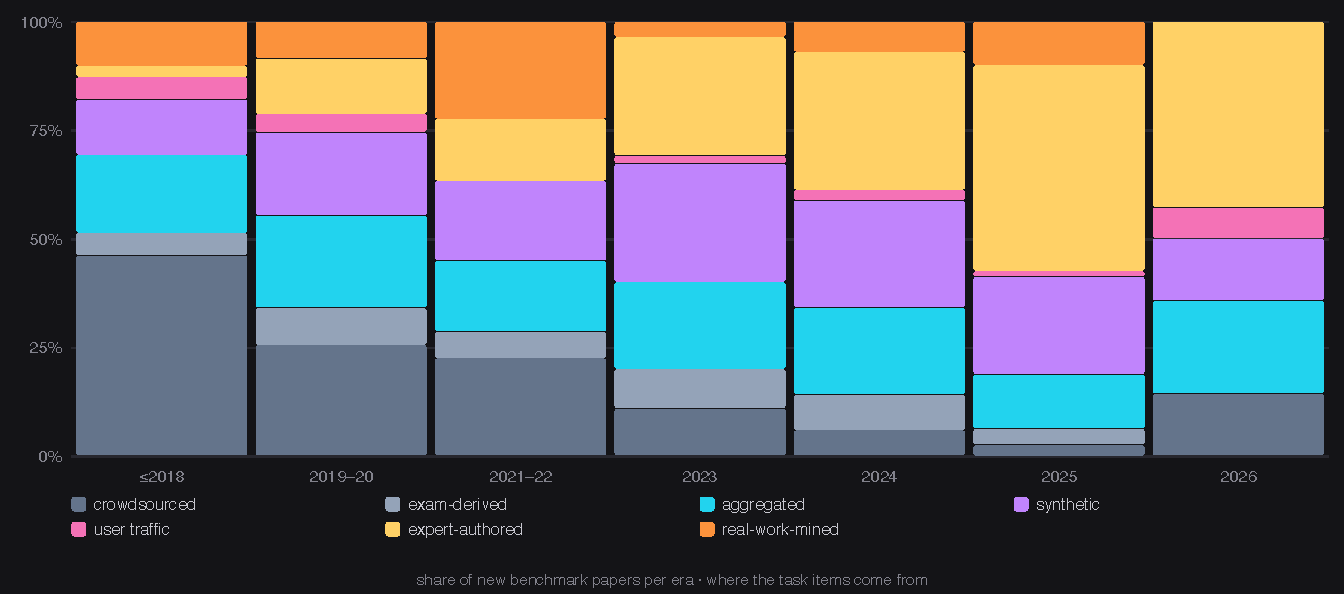
\includegraphics[width=\textwidth]{prov.pdf}
  \caption{Provenance of task items by era. ``Expert-authored'' means items written or
  curated for the benchmark by recruited domain experts; ``real-work-mined'' means harvested
  from artifacts of real work (GitHub issues, freelance jobs, filed contracts).}
  \label{fig:prov}
\end{figure}

Through 2018, benchmarks were built from what could be collected cheaply: crowdworkers and
scraped exams (\TokNCrowdexamTwoZeroOneEight{} of \TokNEraLeTwoZeroOneEight{} papers,
\TokPctCrowdexamLeTwoZeroOneEight\%). By 2025 crowdsourcing has collapsed to
\TokPctCrowdTwoZeroTwoFive\% and \textbf{\TokPctExpertTwoZeroTwoFive\% of new benchmarks are
expert-authored} --- physicians writing HealthBench~\citep{arora-2025-healthbench} criteria,
olympiad medalists writing FrontierMath-class problems, industry professionals with a
fourteen-year average tenure writing GDPval deliverables --- and another
\TokPctRwmTwoZeroTwoFive\% are mined from real work products (SWE-bench's GitHub issues,
SWE-Lancer's~\citep{miserendino-2025-swe-lancer} paid freelance jobs, RLI's~\citep{mazeika-2025-rli}
real projects). The era of the annotation farm is over at the frontier.

The driver is the same as in Section~\ref{sec:waves}: models passed the crowd. When the
evaluated system outperforms a crowdworker at the task, crowd-sourced ground truth stops
being ground truth, item-writing becomes skilled labor, and benchmark construction
industrializes --- which is also why item counts fall as horizons rise. The economics of
expertise, not dataset fashion, is what moved this chart.

\subsection{The contamination cycle}
\label{sec:contam}

\begin{figure}[t]
  \centering
  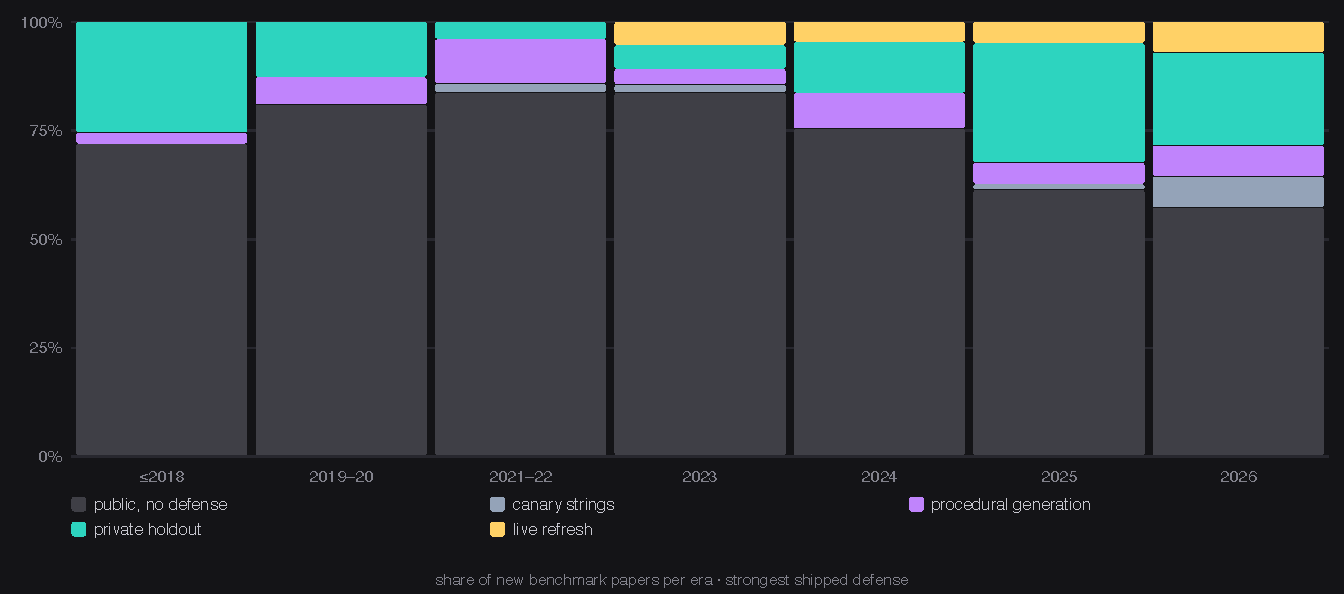
\includegraphics[width=\textwidth]{contam.pdf}
  \caption{Strongest shipped contamination defense by era. ``Private holdout'' includes
  hidden test sets and evaluation servers; ``live refresh'' means post-cutoff or
  continuously regenerated items by design.}
  \label{fig:contam}
\end{figure}

The instructive row is one of the oldest. The corpus's earliest era already had the answer:
\TokNPrivholdTwoZeroOneEight{} of \TokNEraLeTwoZeroOneEight{} papers through 2018
(\TokPctPrivholdLeTwoZeroOneEight\%) shipped a hidden test set or an evaluation server ---
\TokPrivholdLeTwoZeroOneEightEx{} among them --- because a benchmark you could only query
through a leaderboard was the norm when the test set was the scarce asset. The web-scrape
training era then let it lapse: \TokNNonpubTwoOneTwoTwo{} of \TokNEraTwoOneTwoTwo{} papers in
2021--22 published everything (\TokNonpubTwoOneTwoTwoEx{}), leaving only
\TokPctDefTwoOneTwoTwo\% with any defense at all, and the contamination crisis of 2023--24
--- GSM1k~\citep{zhang-2024-gsm1k} measured up to eight points of inflation on GSM8K --- was
the bill for that amnesia. From 2024 the defenses return and diversify: private holdouts
(\TokNPrivholdTwoZeroTwoFive{} of \TokNTwoZeroTwoFive{} papers in 2025,
\TokPctPrivholdTwoZeroTwoFive\%), live refresh
(LiveCodeBench~\citep{jain-2024-livecodebench}, SciPredict's~\citep{sehwag-2026-scipredict}
post-cutoff sourcing), procedural generation (Reasoning
Gym~\citep{stojanovski-2025-reasoning-gym}), and canary strings.

The recovery is real and still partial, and the honest way to state it is as a level, not a
crossing. The share of new benchmarks shipping \emph{some} defense runs
\TokPctDefLeTwoZeroOneEight\% (through 2018) $\rightarrow$ \TokPctDefOneNineTwoZero\%
$\rightarrow$ \TokPctDefTwoOneTwoTwo\% $\rightarrow$ \TokPctDefTwoZeroTwoThree\%
$\rightarrow$ \TokPctDefTwoZeroTwoFour\% $\rightarrow$ \TokPctDefTwoZeroTwoFive\%
$\rightarrow$ \TokPctDefTwoZeroTwoSix\% (\TokNDefTwoZeroTwoSix{} of \TokNTwoZeroTwoSix{} in
2026): a dip and a return, with the 2020s cohorts finally passing the era that invented the
practice --- but \textbf{no era in \TokSpanYears{} years has ever crossed half}, peaking at
\TokPctDefMax\%. The default benchmark, in every era of this corpus, ships public and
undefended.

The defenses also work differently well. Of the \TokNLiverefresh{} live-refresh benchmarks,
\textbf{\TokNSatLiverefresh{} are saturated}; private holdouts saturate at
\TokPctSatPrivhold\%, slightly \emph{above} the corpus base rate of \TokPctSatCorpus\%. A
hidden test set stops leakage but not progress. Refresh-by-design is the only defense that
also buys longevity, which is why the newest entries --- SciPredict's ``no paper before March
2025,'' UpBench's~\citep{yi-2025-upbench} live freelance feed --- build refresh into the
sampling frame rather than bolting privacy onto a frozen set.

\subsection{Horizon is destiny}
\label{sec:destiny}

\begin{figure}[t]
  \centering
  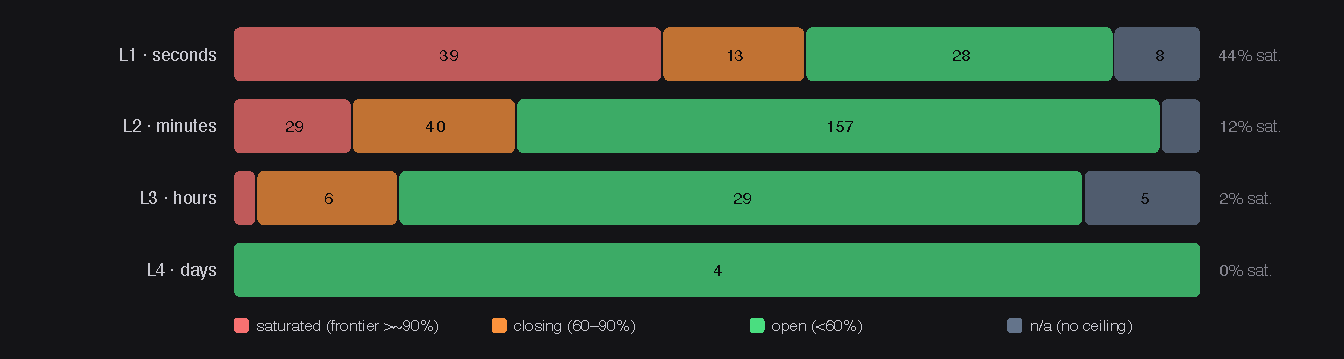
\includegraphics[width=\textwidth]{satbars.pdf}
  \caption{Saturation status by task horizon, judged from the frontier scores each explainer
  quotes (mid-2026). Counts inside bars.}
  \label{fig:satbars}
\end{figure}

Saturation is almost perfectly ordered by the ladder: \textbf{\TokPctSatLOne\% of L1
benchmarks are saturated, \TokPctSatLTwo\% of L2, and \TokPctSatLThreePlus\% of L3 and
above} (Figure~\ref{fig:satbars}). Of the corpus's \TokNSat{} saturated benchmarks,
\TokNSatLThreePlus{} poses a task longer than half an expert-hour ---
\TokSatLThreePlusList{}, a protein-modelling suite whose long tasks are graded against a
numeric answer key. That exception is the rule restated: it is the one shape of long-horizon
benchmark that can saturate, because it never had to pay for open-ended grading. Domain
matters less than one might expect, and defense matters less than refresh
(Section~\ref{sec:contam}); what predicts whether a benchmark is still discriminating in 2026
is simply how much expert time its tasks embody.

That gives builders a clean actuarial rule --- \emph{expected lifespan is bought in
human-minutes per item} --- and it explains the corpus's own shape. The L1 rows are the
field's history; the L2 rows are its present workhorses, \TokPctClosingLTwo\% of them already
closing; the L3--L4 rows, \TokPctOpenLThreePlus\% of which are still open, are where
evaluation currently lives. The ladder of Section~\ref{sec:findings} is not merely being
climbed; it is being consumed from the bottom.

\section{Cross-paper connections}
\label{sec:connections}

The companion page reports nine connections mined by tracing the corpus's internal citation
graph (\TokNEdges{} edges among the \TokN{} papers, plus \TokNLineage{} typed lineage
relations recorded per paper during classification) against the full text of every explainer.
We detail three here, chosen because each sharpens a finding above. Each is visible only
across papers.

\subsection{The audit shadow is not universal}

\begin{figure}[t]
  \centering
  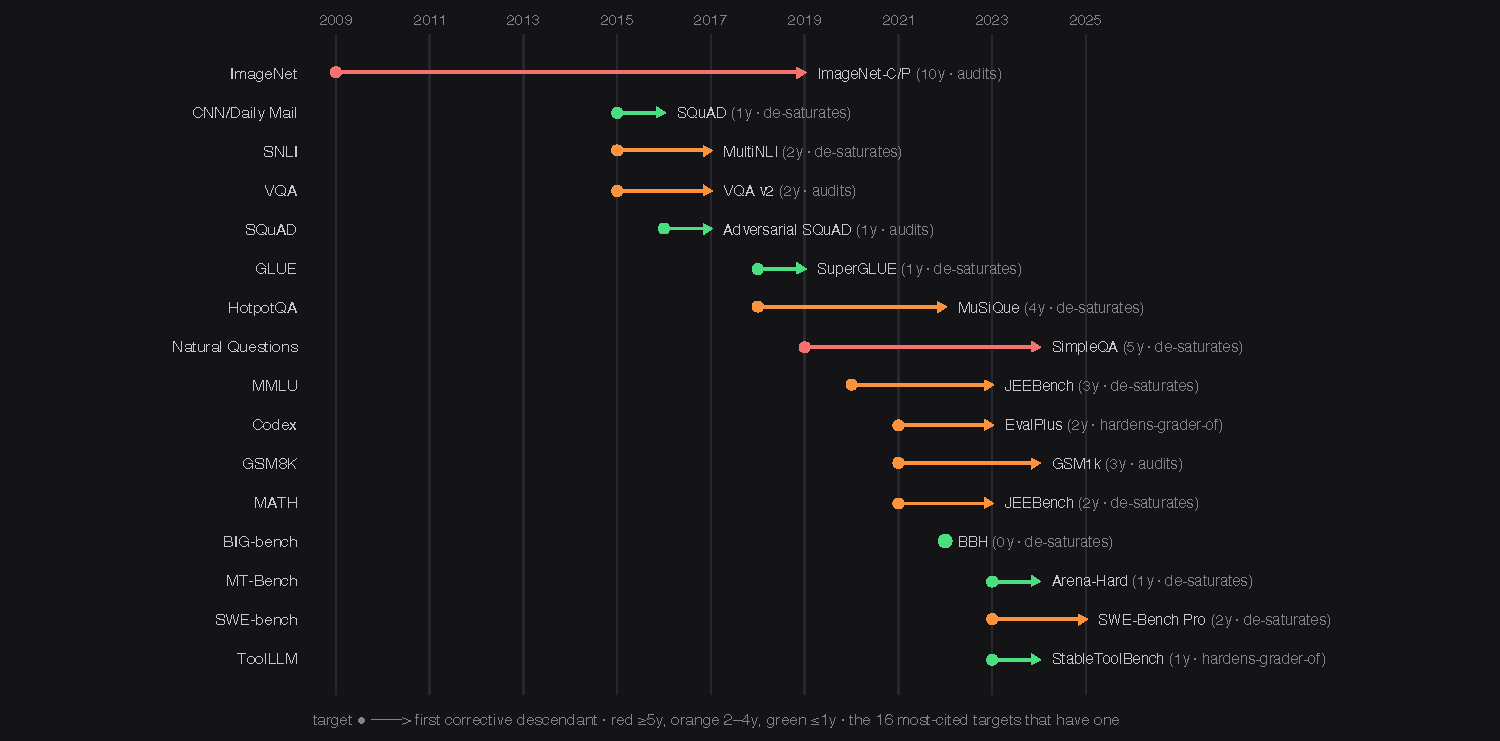
\includegraphics[width=\textwidth]{auditshadow.pdf}
  \caption{First \emph{corrective} descendant of the most-cited targets that have one: a
  child that audits its parent, de-saturates it, or hardens its grader. Extension relations
  (descends-from, responds-to, ports-to-new-domain) are excluded, and the gap between the two
  is the finding.}
  \label{fig:auditshadow}
\end{figure}

Reading the lineage graph for \emph{corrective} descent only turns the audit shadow from a
slogan into a count (Figure~\ref{fig:auditshadow}). \TokNCorrections{} such edges exist among
the \TokN{} papers, reaching \TokNAudited{} distinct targets, and the longest unaudited
stretch in the corpus is \TokLagMaxPair{} at \TokLagMax{} years. The wait has been
shortening: the longest first-correction lag is \TokLagMaxLeTwoZeroOneEight{} years for
targets published through 2018, \TokLagMaxOneNineTwoZero{} for 2019--20 targets,
\TokLagMaxTwoOneTwoTwo{} for 2021--22, and \TokLagMaxTwoThreeTwoFour{} for 2023 and later
(medians \TokLagMedLeTwoZeroOneEight{}, \TokLagMedOneNineTwoZero{},
\TokLagMedTwoOneTwoTwo{}, \TokLagMedTwoThreeTwoFour{}). Part of that is real and part of it
is arithmetic --- a 2024 benchmark \emph{cannot} have a five-year-old audit yet --- so the
honest version of the claim is the one the early rows carry on their own: the pre-2019 cohort
contains both a one-year correction and a ten-year one, and the recent cohorts contain no
long waits at all.

The stronger claim, that every benchmark which mattered eventually acquired an audit, is
false, and the graph is what falsifies it. \textbf{Of the corpus's twenty most-cited
benchmarks, \TokNTopTwoZeroAudited{} have a corrective descendant here.} The rest ---
\TokTopTwoZeroUnauditedEx{} among them --- have plenty of descendants, but those descendants
\emph{extend} rather than correct: new domains, new modalities, harder instances of the same
format. Correction and extension are different evolutionary pressures, and the agent-era
gravity wells have so far attracted mostly the second. That is worth watching, because
extension inherits a benchmark's construct without ever testing it.

Where the shadow does fall, its mechanism has changed. Early corrections were third-party
forensics --- a Berkeley group rebuilding ImageNet's test
set~\citep{recht-2019-imagenet-generalize} --- but by 2024--25 they moved in-house and turned
pre-emptive: OpenAI hardened its own SimpleQA~\citep{wei-2024-simpleqa} into
BrowseComp~\citep{wei-2025-browsecomp}, LMSYS distilled its own arena into
Arena-Hard~\citep{li-2024-arena-hard}, Scale extended its own MultiChallenge into an audio
twin. Quality control became contemporaneous with publication. Read from the supply side,
this is the same lifespan clock as Section~\ref{sec:destiny}: the shorter a benchmark's
discriminating life, the sooner its successor must already be in press.

\subsection{The benchmark is the reward}
\label{sec:reward}

The canonical benchmarks were never eval-only artifacts. GSM8K shipped as verifier-training
infrastructure --- a 7.5K training split plus a learned verifier, with the launch paper
already documenting that verifier being reward-hacked.
HumanEval~\citep{chen-2021-codex} arrived inside the Codex training paper, its unit tests
doubling as a sample-selection oracle; SWE-bench shipped 19K training instances and its own
fine-tunes. When GSM1k later audited the ecosystem, its most telling overfitting case was
contaminated through the \emph{grader lineage} --- a process-reward model leaking reasoning
chains --- with no test-set leak an $n$-gram checker could see.

Validity then had to be re-purchased, each time by moving the grader further from the
training corpus: EvalPlus~\citep{liu-2023-evalplus} densified HumanEval's tests roughly
eightyfold; SWE-bench Pro~\citep{deng-2025-swe-bench-pro} bought commercial code models could
never have seen, and its 25-to-30-point public-to-commercial score collapse --- same models,
same harness --- is the field's cleanest single measurement of what training against a public
grader family costs. By 2025 the flip is doctrine:
MLGym's~\citep{nathani-2025-mlgym} complaint about prior benchmarks is that they
\emph{cannot} be trained on, and Reasoning Gym publishes its reward function outright.
Goodhart does not vanish under procedural generation; it migrates into the grader's blind
spots.

\subsection{Gravity selects portability}

APPS~\citep{hendrycks-2021-apps} and HumanEval are same-year, mutually citing,
execution-graded code benchmarks; APPS was some sixty times larger, with twice the tests per
problem. Yet HumanEval's paper is the most-cited node in this corpus ---
\TokGravHumaneval{} in-corpus citations, ahead of \TokGravRunnerup{}'s
\TokGravRunnerupN{} and against APPS's \TokGravApps{} --- because what the field reused was
the \emph{measurement kit}: the unbiased pass@$k$ estimator plus 164 cheap, self-contained
tasks scoring in the discriminative range. APPS's grader vocabulary failed to travel (its
lenient metric flattered; its strict metric floored at zero on the whole competition tier).
The clincher: when EvalPlus proved HumanEval's thin tests inflate pass@$k$ by up to about
29\%, the field patched HumanEval in place rather than migrate to APPS --- which already had
denser tests.

The pattern repeats a generation down. SWE-bench Pro's forkable Docker harness is already
substrate for third-generation benchmarks, while SWE-Lancer's more rigorous but unforkable
grader --- triple-verified end-to-end tests on one proprietary repository --- has
\TokNSwelDescCoding{} coding descendants. Every benchmark that descends from it
(\TokSwelDescList{}) took the \emph{framing}, real-dollar difficulty, into the
economic-rehearsal family instead, and the coding benchmarks that cite it do so to explain
what they did differently. Benchmark genes travel through cheap, reproducible harnesses: the
ecosystem structurally selects reproducibility over rigor.

\section{Method and caveats}
\label{sec:method}

\paragraph{Corpus.}
\label{sec:intro-rubric}
The \TokN{} papers are the atlas's \texttt{benchmarks} survey tag, applied when each paper
joined the atlas under the headline-contribution rubric of Section~\ref{sec:facets}. The set
over-represents what the atlas covers deeply --- language-model, agent, and safety evaluation
from 2023 onward, which is \TokNTwoZeroTwoThree{} + \TokNTwoZeroTwoFour{} +
\TokNTwoZeroTwoFive{} + \TokNTwoZeroTwoSix{} of the \TokN{} --- and samples the earlier
generations rather than enumerating them, so era-level trends should be read as trends
\emph{within this kind of corpus}, not a census of all benchmarks ever built. The corpus is
papers only; the 2026 model-card canon also includes non-paper instruments this survey does
not cover (SWE-bench Verified, Aider Polyglot, AIME-as-eval, the ARC-AGI leaderboards,
needle-in-a-haystack probes), an exclusion of form rather than a judgment that they do not
matter.

\paragraph{Classification.} Each paper was classified from its atlas explainer (and the paper
itself where the explainer underdetermined a dimension) by a language-model pipeline, in two
historical stages. The first 139 papers got one full-schema pass followed by a fully
independent second pass re-classifying the six judgment-heavy dimensions with different paper
groupings; the two passes agreed on 94.8\% of the 750 compared values, and all 39
disagreements, on 32 papers, were adjudicated by a third read of the source text, with
saturation the noisiest dimension (16 of the 39 conflicts). The remaining 230 were classified
in a later backfill, sharded into 12 batches of roughly 20 against the same schema, then
merged, after which in-corpus citation in-degree was recomputed across the whole corpus and
the lineage graph re-enriched --- a shard can only see the papers inside it. Those two stages
did not get equal scrutiny and the record carries the difference: \TokNConfMed{} of \TokN{}
records are marked \texttt{confidence: medium}. Treat individual facet values --- saturation
above all --- as softer than any aggregate here.

\paragraph{Tree placement.} Kingdom and family addresses were assigned by the same protocol,
judging role at birth from each paper's own problem statement, with lineage restricted to
relations between papers both in the corpus (\TokNLineage{} of them, over \TokNEdges{}
citation edges among the \TokN{}). The independent second placement pass covered 78 papers of
the original 139-paper corpus before rate-limiting and disagreed on 5 placements, each
re-adjudicated against the source text. Two known lineage biases run in the same direction:
a shard could not link to a parent sitting in a sibling shard (the post-merge enrichment pass
exists to repair that, and did, but cannot prove it caught everything), and because a node's
date is its arXiv v1 month while its camera-ready cites later work, genuinely
forward-pointing relations were dropped rather than recorded. The lineage graph therefore
understates connectivity, in both cases arbitrarily with respect to the subject matter.

\paragraph{Connections.} The connection stories were mined by lens-directed search over the
corpus and its citation graph, then verified two ways: every quotation was checked against
the explainer texts, and every citation-structure assertion (``X cites Y,'' ``X and Y share
no edge'') was checked mechanically against the graph. Claims that survived only partially
were corrected or dropped; the numbers inside the stories are the source papers' own.

\paragraph{Known soft spots.} Task-horizon rungs are estimates of the \emph{typical} instance
from the papers' own task descriptions; only a few papers measure human time directly.
Saturation reflects the frontier scores quoted in each explainer through mid-2026, and it
ages. The recorded grading family is the headline metric only; many benchmarks ship secondary
graders. Item counts are approximate. The domain vocabulary cannot name robotics, multi-agent
reinforcement learning, or theory of mind, all of which the corpus contains, so any
domain-sliced number inherits that squeeze. And one dimension a future pass should add is
whether each benchmark's grader was itself adversarially audited --- the agentic-benchmark
checklist's 7-of-10 finding suggests that column would be mostly empty.

\section{Conclusion}

Placed in a single structure, \TokN{} benchmarks stop looking like a scoreboard and start
looking like an ecosystem governed by one economics. A benchmark can only pose tasks as long
as it can afford to grade them, so the reach of evaluation is bounded by the cost of its
grader; the verifiable, cheap-to-grade benchmarks are also the reward functions models train
against; and a benchmark's lifespan is bought in human-minutes per item, which is why the
field is climbing the horizon ladder and consuming it from the bottom at the same time.
Capability probes --- the thing ``benchmark'' usually connotes --- are already a minority of
what the field builds each year (\TokPctCapTwoZeroTwoFive\% of 2025), the rest auditing,
rehearsing, walling off, and manufacturing signal in a reflexive ecosystem a topic-based
taxonomy cannot see. Two of this survey's corrections to its own earlier, smaller version
generalize past it: a long tail of pre-LLM work (\TokNPreTwoZeroTwoOne{} papers,
\TokPctPreTwoZeroTwoOne\% of the corpus) turns several apparent arrivals into returns, and
reading a lineage graph for \emph{corrective} rather than merely descendant edges turns a
universal claim about auditing into \TokNTopTwoZeroAudited{} of twenty. The corpus, every
figure, and every statistic in this paper are generated from the live companion survey and
regenerate deterministically as the corpus grows.

\bibliographystyle{plainnat}
\bibliography{refs}

\end{document}
